\documentclass[final,smallcondensed]{llncs}

% Geometry
\usepackage{geometry}
\geometry{
  letterpaper,     % or a4paper
  textwidth=15.2cm,  % llncs has 12.2cm
  textheight=22.3cm, % llncs has 19.3cm
  heightrounded,   % integer number of lines
  hratio=1:1,      % horizontally centered
  vratio=2:3,      % not vertically centered
}

\usepackage{graphicx}
\usepackage{makecell}

\begin{document}

\title{Quantstamp: A decentralized security platform for smart contracts}

\author{Steven Stewart \and Richard Ma}

\institute{Quantstamp Technologies Inc.\\\email{info@quantstamp.com}}

\date{\today}

\maketitle

% INTRODUCTION
\section{Overview}
The Quantstamp ({\bfseries QSP}) platform is an automated service, based on blockchain technology, for performing security audits of smart contracts. QSP maintains a history of security reports that are generated whenever an audit of a smart contract is requested. The Quantstamp network ({\bfseries QN}) stores all reports in a decentralized database, which is updated by decentralized consensus. The QSP token is the key to accessing the software services offered by Quantstamp.

Our platform for verification rewards participants who provide compute resources for performing security checks on smart contracts. These checks make up the \emph{security library} and are run by decentralized verifiers in our network. The Quantstamp protocol ensures the verification and certification of smart contracts is part of the mathematical problem that a verifier needs to solve. Quantstamp tokens are the API keys that are used to access the platform. When submitting smart contracts for checking by the network, the dynamic token transaction fee that is attached to the submission accounts for supply and demand on the QN. 

The utility of QSP is best illustrated by example. Suppose a developer plans to deploy a smart contract written in Solidity on Ethereum. There is substantial risk when writing code that accesses a monetary system, and the developer must be careful to ensure that no funds are lost due to vulnerabilities. In order to minimize risk, the developer submits his code for a security audit, and calls the auditing function directly from his wallet by sending a small amount of QSP token to the QN network. Then, the QN broadcasts the audit request and verifiers immediately perform a set of security checks. Upon consensus, the network publishes a security report that summarizes the results. The report classifies issues based on a severity system from 1--10; a 1 is a minor warning, a 10 is a major vulnerability. 

When requesting an audit, the developer can choose either a public or private security report. Private reports are encrypted using the public key of the smart contract and can be decrypted by the owner/developer. By using seamless cryptographic hashing, security reports viewed by the public exactly match the audited source code to prevent manipulation of report results.

A developer can perform security audits on a local machine prior to issuing a public audit, but may find that the computational overhead is too high. Verifier nodes in the QN are likely to have greater computational capacity in terms of memory and processing cores than the average developer's machine. Once the code is ready for deployment, the developer is ultimately motivated to produce a public security report in order to give users the reassurance that a decentralized security audit was performed.

When a security report identifies issues found within a smart contract, the developer has the option of publicly annotating the report with feedback. This gives developers the power to indicate false-positives in the report, and the community can validate the annotations.

Although it is not possible to 100\% guarantee that source code is flawless, the Quantstamp team will continuously engage in research and development, making regular improvements to the security library. When there are new releases, developers can re-audit their smart contracts, demonstrating their commitment to securing code and increasing public confidence.


\section{Token distribution}

\subsection{The Quantstamp Presale (100\% bonus)}

\begin{table}[]
\begin{tabular}{| l | l |}
\hline
\makecell[lt]{\textbf{Presale Token}\\QSPG} & \makecell[lt]{\textbf{Type}\\Ethereum ERC20 Token} \\ \hline
\makecell[lt]{\textbf{Price (Includes 100\% bonus)}\\10,000 QSPG = 1 ETH} & \makecell[lt]{\textbf{Issuance} \\QSPG contributions are pre-allocated at the\\start of the main ICO with bonus included} \\ \hline
\makecell[lt]{\textbf{Sale Period}\\Currently taking pre-orders\\First token sale date TBD following full \\regulatory compliance
} & \makecell[lt]{\textbf{Early Backer Reward}\\Bonus starts at 100\% in the first 48 hours,\\then linearly decreases to 50\% over one\\month} \\ \hline
\end{tabular}
\end{table}

\noindent The github code for our token distribution: https://github.com/quantstamp/token-distribution

\subsection{Main Token Sale Terms}

\begin{figure}[h!]
  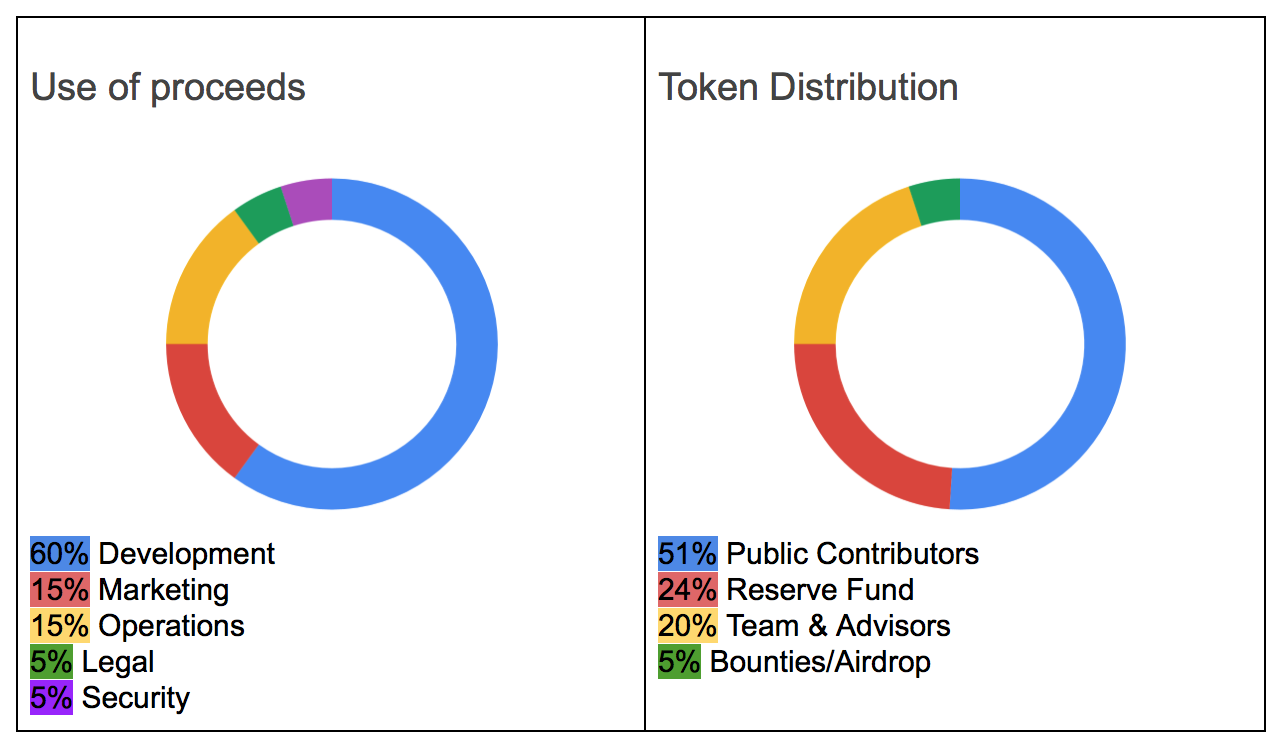
\includegraphics[scale=0.45]{token_sale.png}
\end{figure}

\begin{table}[h!]
\begin{tabular}{|l|l|}
\hline
Role of Token           & Enable security audits on the Quantstamp Network       \\ \hline
Symbol                  & QSP                                                    \\ \hline
Supply                  & 1,000,000,000 QSP                                      \\ \hline
For Sale                & 510,000,000 QSP                                        \\ \hline
Emission Rate           & No new tokens will be created                          \\ \hline
Price                   & 5,000 QSP = 1 ETH                                      \\ \hline
Accepted Currencies     & ETH                                                    \\ \hline
Sale Period             & November 2017                                          \\ \hline
Token Distribution Date & 7 days following security audits at the end of the ICO \\ \hline
Minimum Goal            & 5000 ETH                                               \\ \hline
Maximum Goal            & 102,000 ETH                                            \\ \hline
\end{tabular}
\end{table}

\noindent Additional information regarding the token distribution is in the FAQ section of our white-paper.

\end{document}
